\documentclass[11pt, a4paper]{article}
\usepackage{pdfpages}
\usepackage{parallel}
\usepackage[T2A]{fontenc}
\usepackage{ucs}
\usepackage[utf8x]{inputenc}
\usepackage[polish,english,russian]{babel}
\usepackage{hyperref}
\usepackage{rotating}
\usepackage[inner=2cm,top=1.8cm,outer=2cm,bottom=2.3cm,nohead]{geometry}
\usepackage{listings}
\usepackage{graphicx}
\usepackage{wrapfig}
\usepackage{longtable}
\usepackage{indentfirst}
\usepackage{array}
\usepackage{tikzsymbols}
\usepackage{soul}
\usepackage[ruled,vlined]{algorithm2e}
%\counterwithout{figure}{section} 

\usepackage{url}
\makeatletter
\g@addto@macro{\UrlBreaks}{\UrlOrds}
\makeatother

\newcolumntype{P}[1]{>{\raggedright\arraybackslash}p{#1}}
\frenchspacing
\usepackage{fixltx2e} %text sub- and superscripts
\usepackage{icomma} % коскі ў матэматычным рэжыме
\PreloadUnicodePage{4}

\newcommand{\longpage}{\enlargethispage{\baselineskip}}
\newcommand{\shortpage}{\enlargethispage{-\baselineskip}}

\def\switchlang#1{\expandafter\csname switchlang#1\endcsname}
\def\switchlangbe{
\let\saverefname=\refname%
\def\refname{Літаратура}%
\def\figurename{Іл.}%
}
\def\switchlangen{
\let\saverefname=\refname%
\def\refname{References}%
\def\figurename{Fig.}%
}
\def\switchlangru{
\let\saverefname=\refname%
\let\savefigurename=\figurename%
\def\refname{Литература}%
\def\figurename{Рис.}%
}

\hyphenation{admi-ni-stra-tive}
\hyphenation{ex-pe-ri-ence}
\hyphenation{fle-xi-bi-li-ty}
\hyphenation{Py-thon}
\hyphenation{ma-the-ma-ti-cal}
\hyphenation{re-ported}
\hyphenation{imp-le-menta-tions}
\hyphenation{pro-vides}
\hyphenation{en-gi-neering}
\hyphenation{com-pa-ti-bi-li-ty}
\hyphenation{im-pos-sible}
\hyphenation{desk-top}
\hyphenation{elec-tro-nic}
\hyphenation{com-pa-ny}
\hyphenation{de-ve-lop-ment}
\hyphenation{de-ve-loping}
\hyphenation{de-ve-lop}
\hyphenation{da-ta-ba-se}
\hyphenation{plat-forms}
\hyphenation{or-ga-ni-za-tion}
\hyphenation{pro-gramming}
\hyphenation{in-stru-ments}
\hyphenation{Li-nux}
\hyphenation{sour-ce}
\hyphenation{en-vi-ron-ment}
\hyphenation{Te-le-pathy}
\hyphenation{Li-nux-ov-ka}
\hyphenation{Open-BSD}
\hyphenation{Free-BSD}
\hyphenation{men-ti-on-ed}
\hyphenation{app-li-ca-tion}

\def\progref!#1!{\texttt{#1}}
\renewcommand{\arraystretch}{2} %Іначай формулы ў матрыцы зліпаюцца з лініямі
\usepackage{array}

\def\interview #1 (#2), #3, #4, #5\par{

\section[#1, #3, #4]{#1 -- #3, #4}
\def\qname{LVEE}
\def\aname{#1}
\def\q ##1\par{{\noindent \bf \qname: ##1 }\par}
\def\a{{\noindent \bf \aname: } \def\qname{L}\def\aname{#2}}
}

\def\interview* #1 (#2), #3, #4, #5\par{

\section*{#1\\{\small\rm #3, #4. #5}}
\ifx\ParallelWhichBox\undefined%
    \addcontentsline{toc}{section}{#1, #3, #4}%
\else%
\ifnum\ParallelWhichBox=0%
    \addcontentsline{toc}{section}{#1, #3, #4}%
\fi\fi%

\def\qname{LVEE}
\def\aname{#1}
\def\q ##1\par{{\noindent \bf \qname: ##1 }\par}
\def\a{{\noindent \bf \aname: } \def\qname{L}\def\aname{#2}}
}

\newcommand{\interviewfooter}[1]{
\vskip 1em
\noindent \textit{#1}
}

\switchlang{ru}
\begin{document}

\title{1989 "--- Kraft trackball}
\date{}
\maketitle
\selectlanguage{russian}
Kraft trackball, известный также как Kraft TripleTrack \cite{triple} "---	 это трекбол, разработанный в конце 80-х годов компанией Kraft Systems, и выпускавшийся для нескольких семейств компьютеров: IBM PC, Atari ST, Commodore 64 и Amiga. К особенностям трекбола можно отнести переключатель блокировки кнопок для выбора и дополнительную съемную педаль.

\begin{figure}[h]
    \centering
    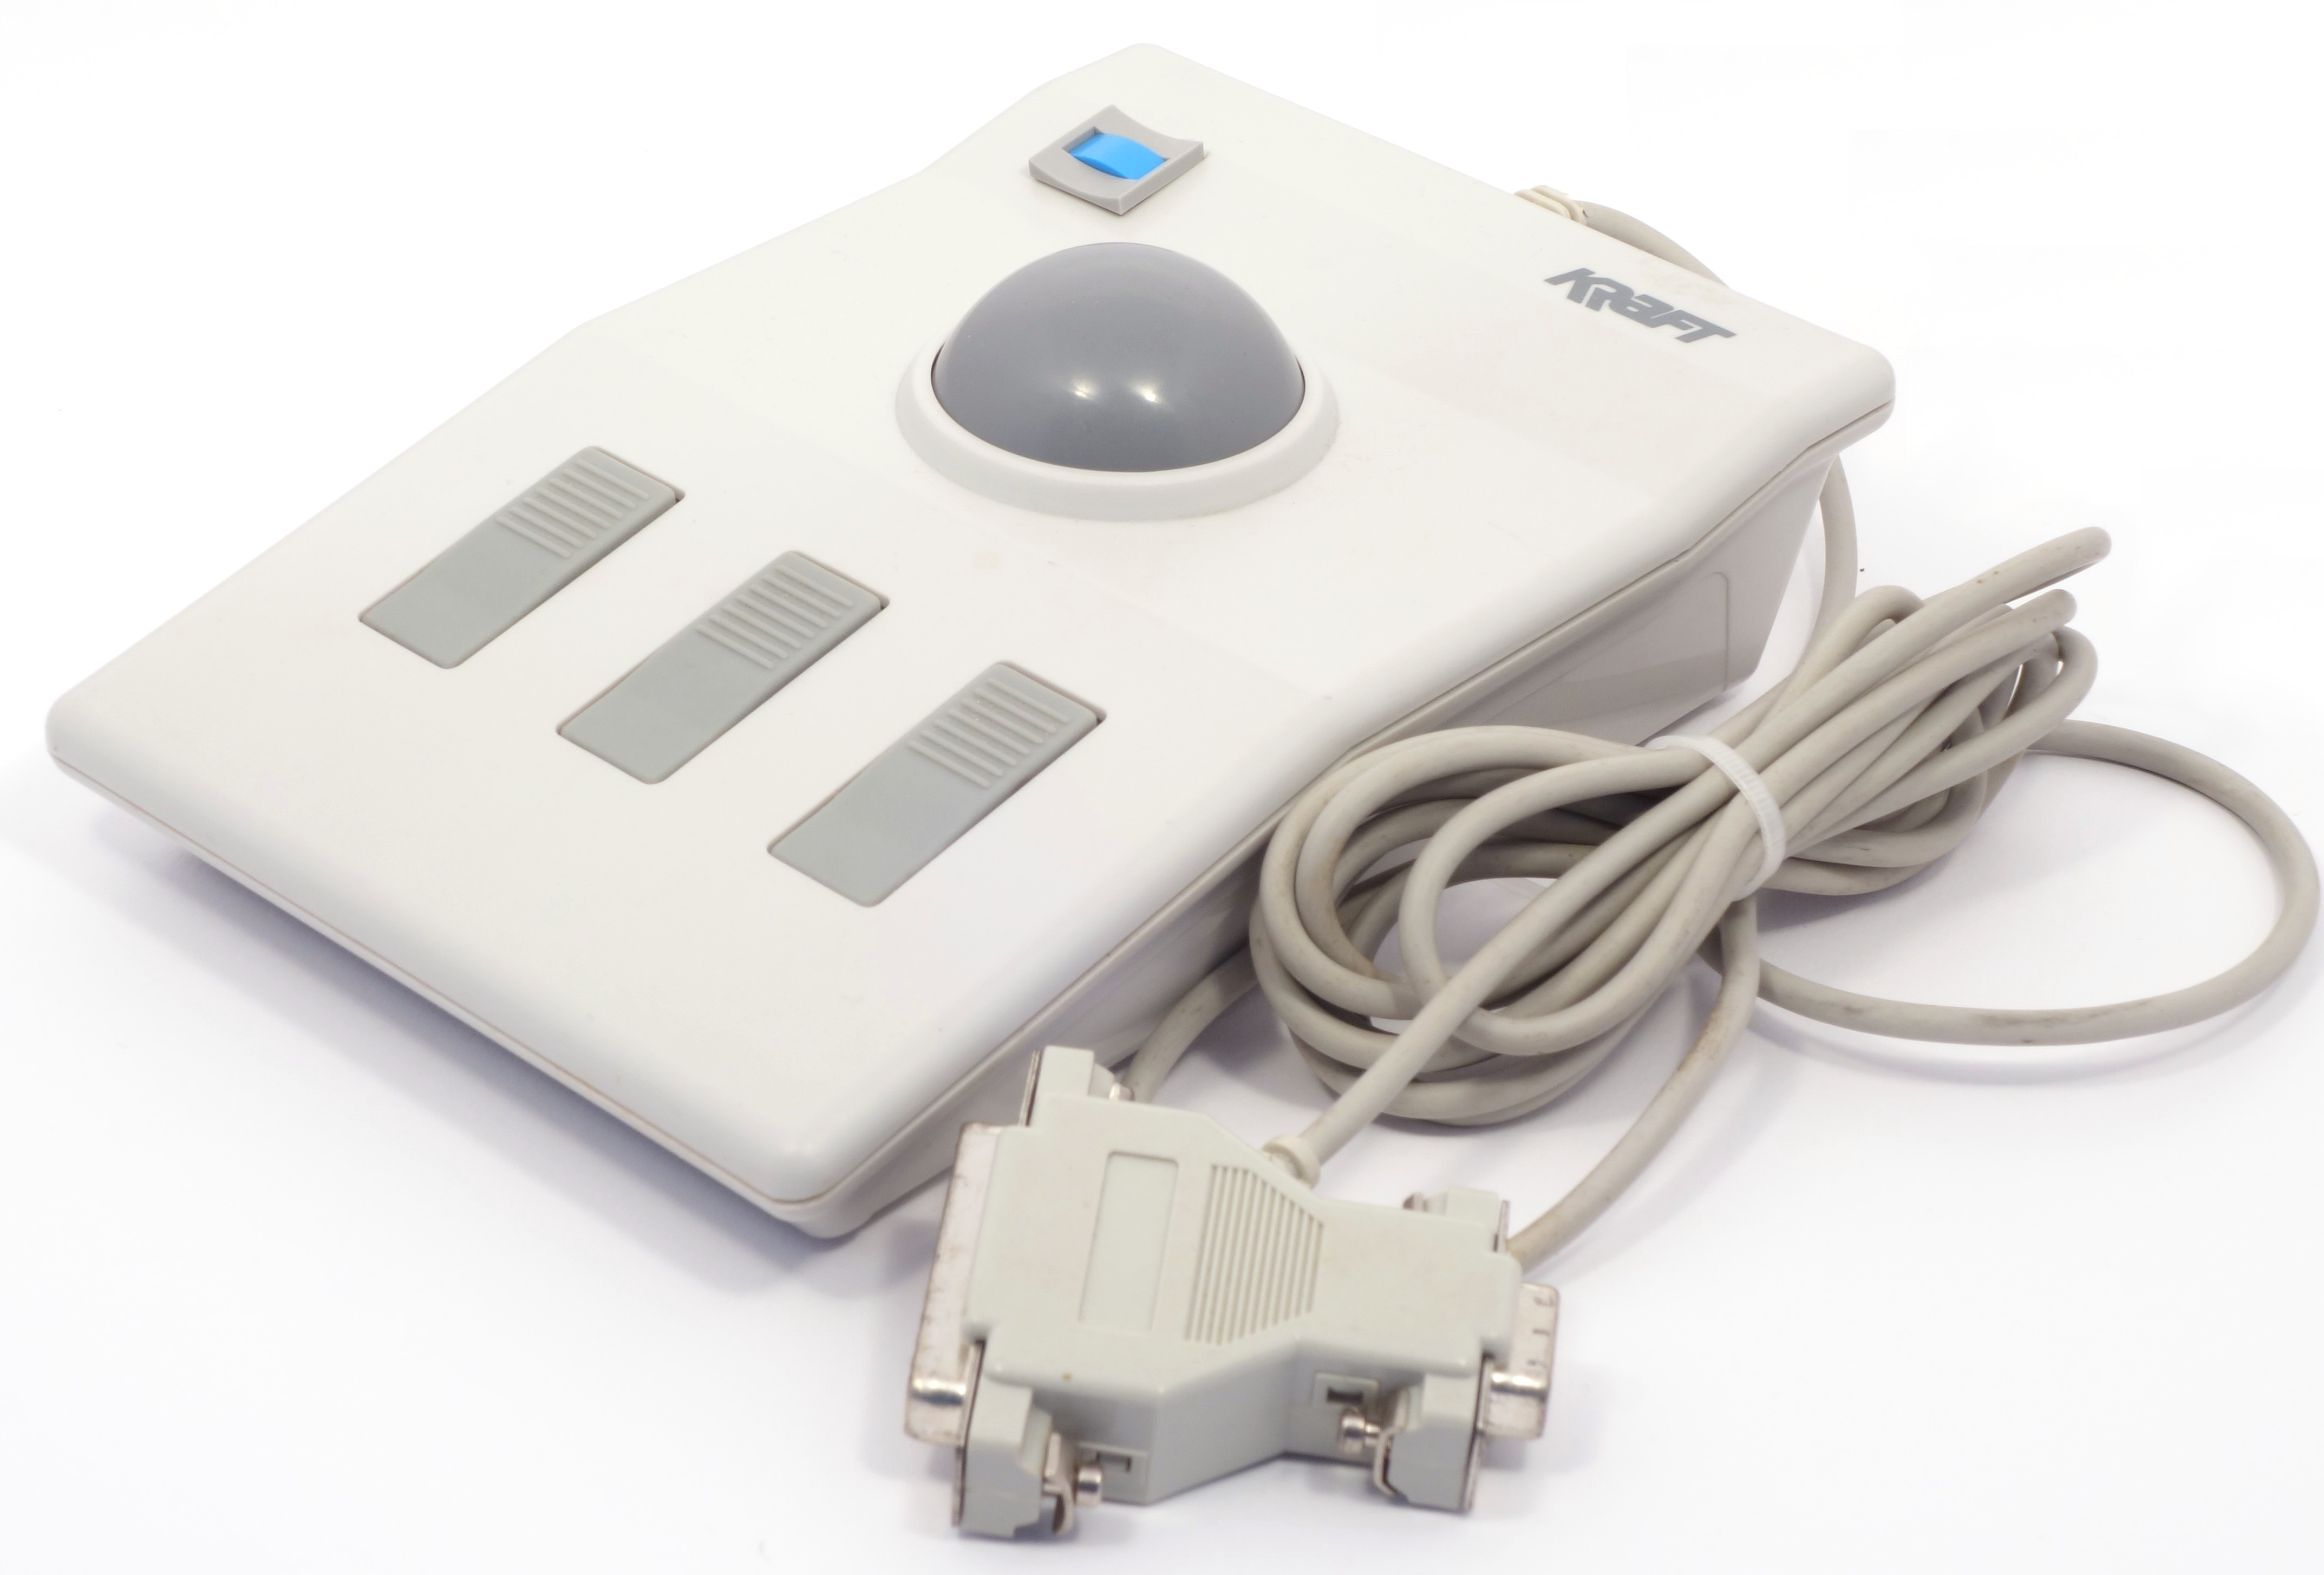
\includegraphics[scale=0.4]{1989_kraft_trackball/pic_30.jpg}
    \caption{Изображение Kraft trackball}
    \label{fig:KraftPhoto}
\end{figure}

Kraft trackball имеет симметричный корпус, и поэтому подходит как для левшей, так и для правшей. Три кнопки расположены на ближней к пользователю части устройства, поэтому трекбол не предлагает никакой опоры под запястье. Центральная кнопка действует как стандартная правая кнопка мыши. Кнопки построены на основе качественных переключателями с различимым кликом; однако из-за достаточно большого хода колпачки кнопок при нажатии уходят вглубь, из-за чего их сложнее нажимать большим пальцем.

\begin{figure}[h]
    \centering
    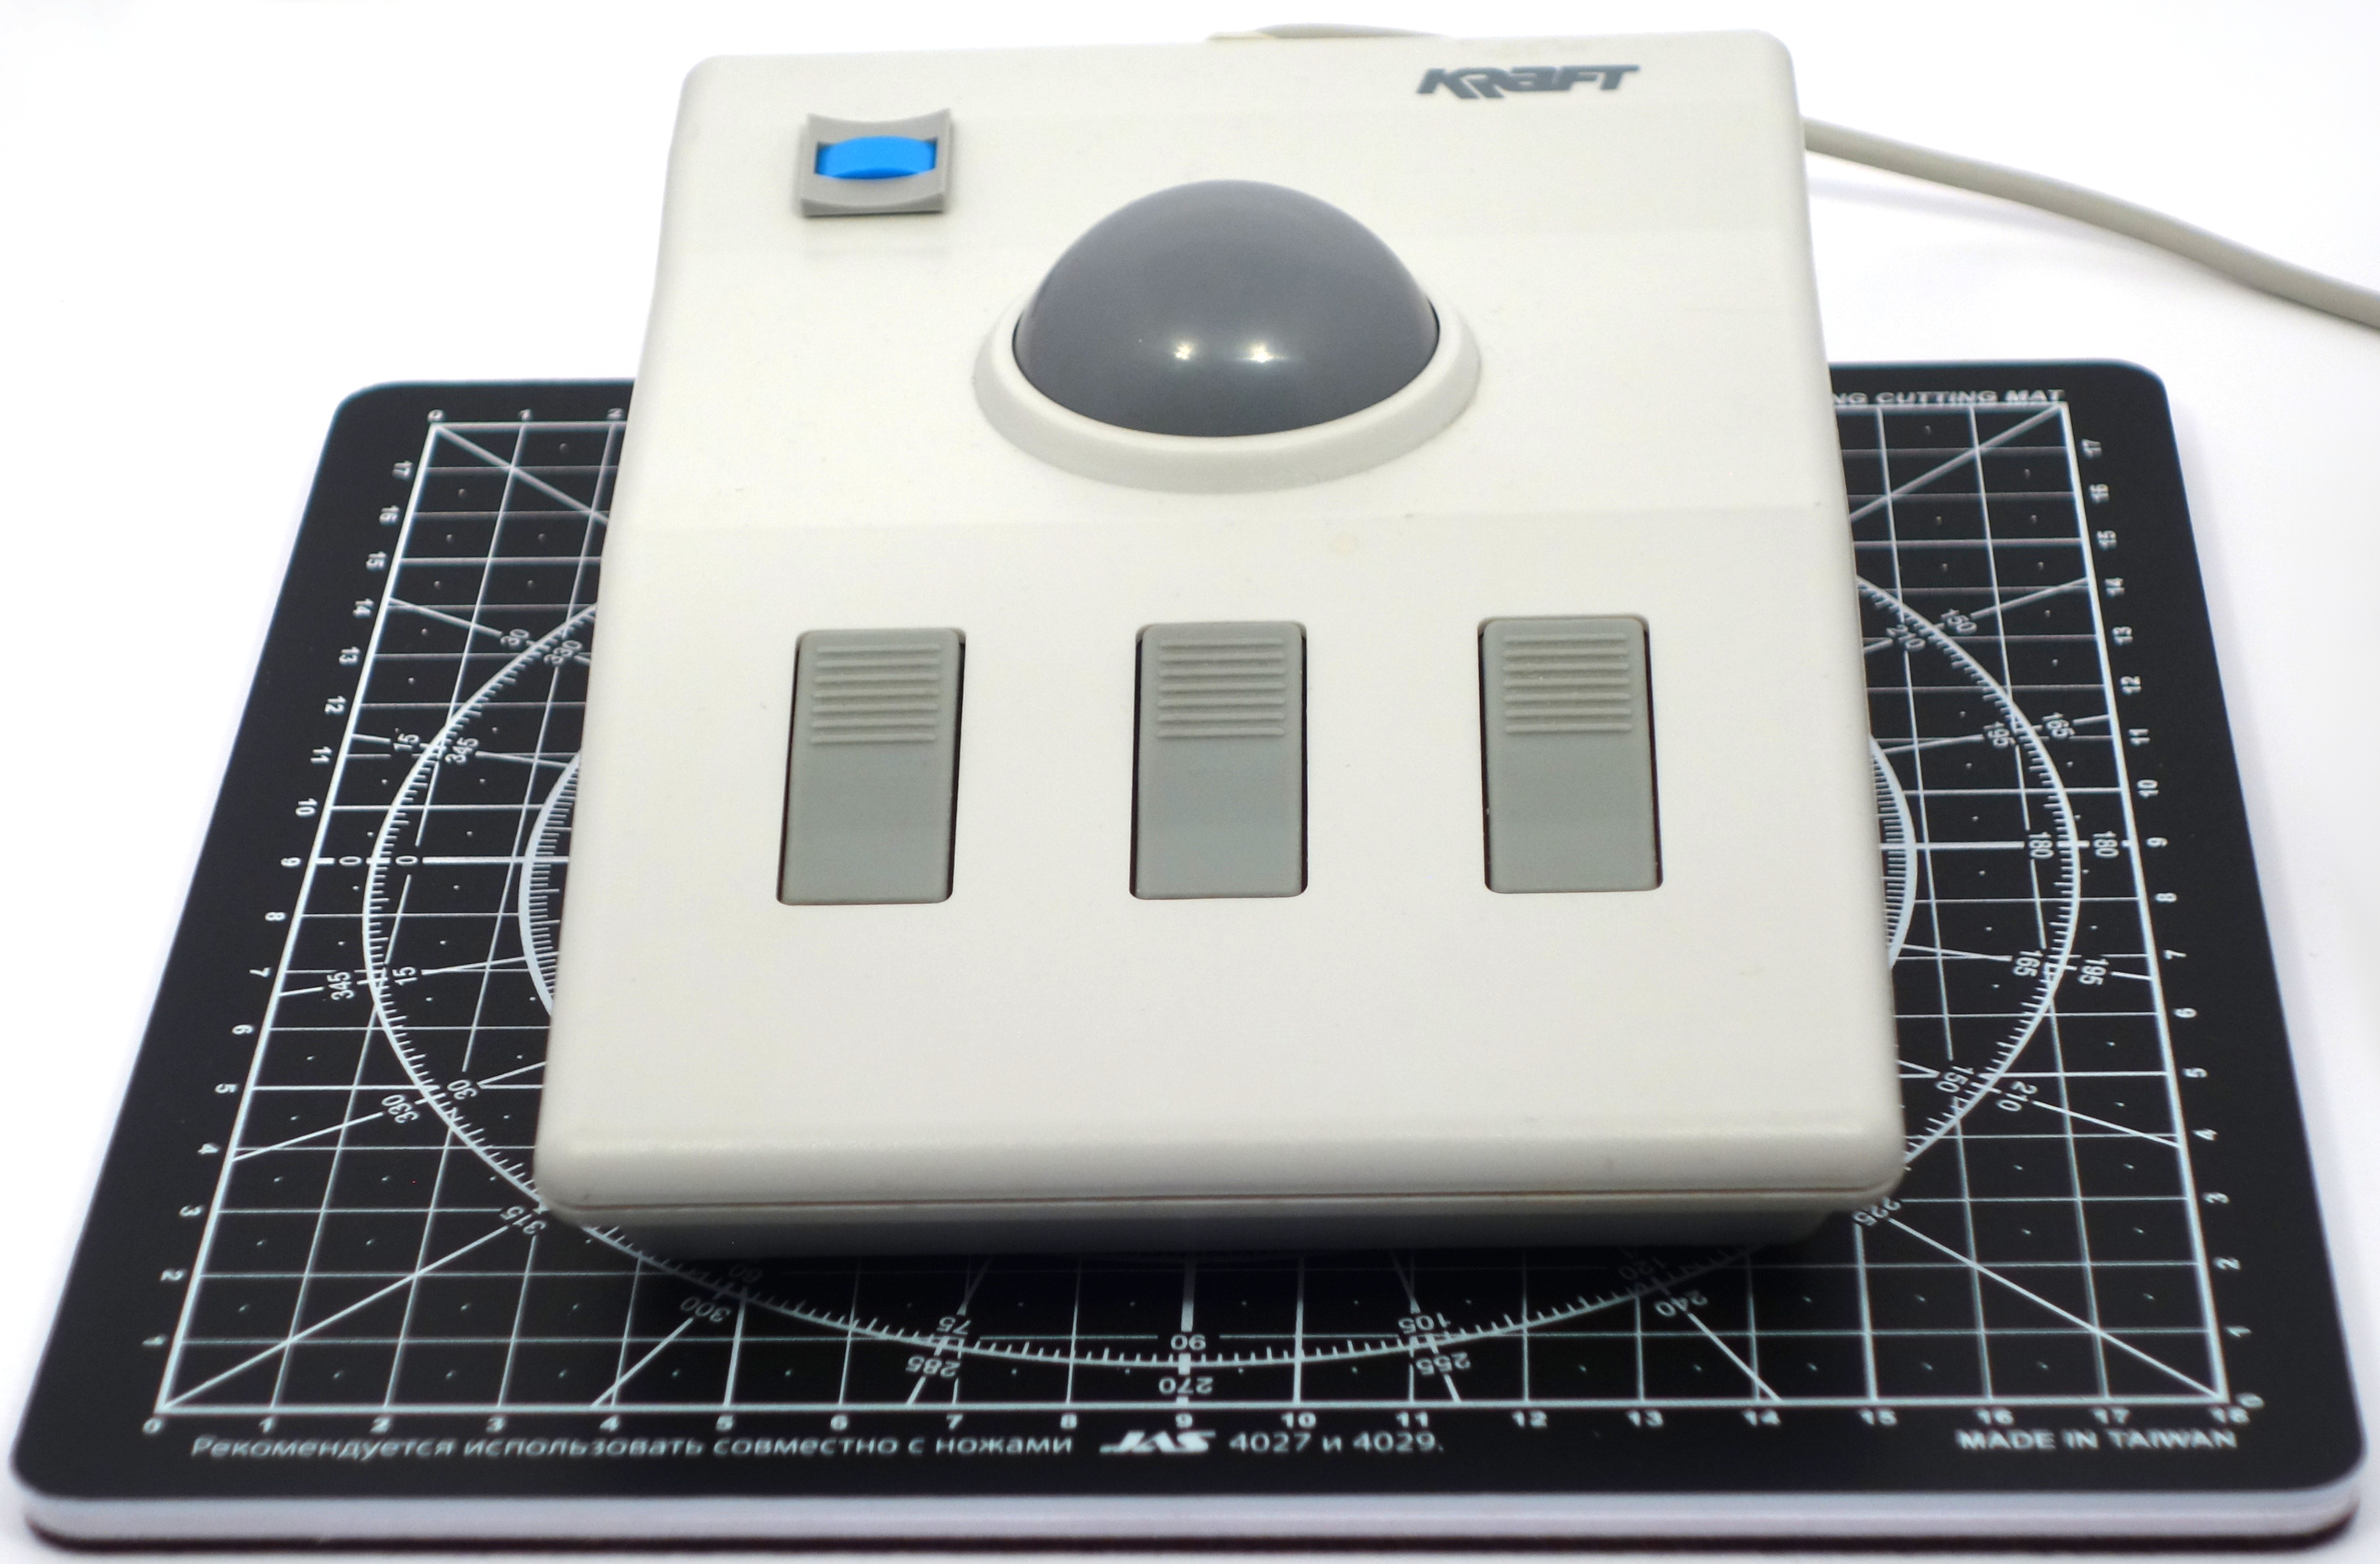
\includegraphics[scale=0.25]{1989_kraft_trackball/size_30.jpg}
    \caption{Изображение Kraft trackball на размерном коврике с шагом сетки 1~см}
    \label{fig:KraftSize}
\end{figure}

Шар имеет хорошую подвижность, поэтому проблем в управлении курсором у устройства нет. При этом часть с шаром несколько приподнята над кнопками, что можно расценивать в плане эргономики как преимущество.

В \cite{Hudnall} отмечается простота установки идущего в комплекте программного обеспечения, а также выделены две проблемы в управлении курсором с помощью этого трекбола: кнопки нажимаются сложнее, чем, например, кнопки у популярных моделей мышей, а также иногда происходит проскальзывание шара (курсор остается на месте). Последняя проблема решается пользователем с помощью быстрого возвратно-поступательного движения. В целом, поместив средний палец на шар, а большой палец на крайнюю левую кнопку (рис. \ref{fig:KraftHand}), получается довольно легко перемещать курсор по экрану. Использование правой или средней кнопки менее естественно в анатомическом плане, к нему сложнее привыкнуть, и, к счастью для пользователя, в конце восьмидесятых годов это требовалось не так часто.

\begin{figure}[h]
    \centering
    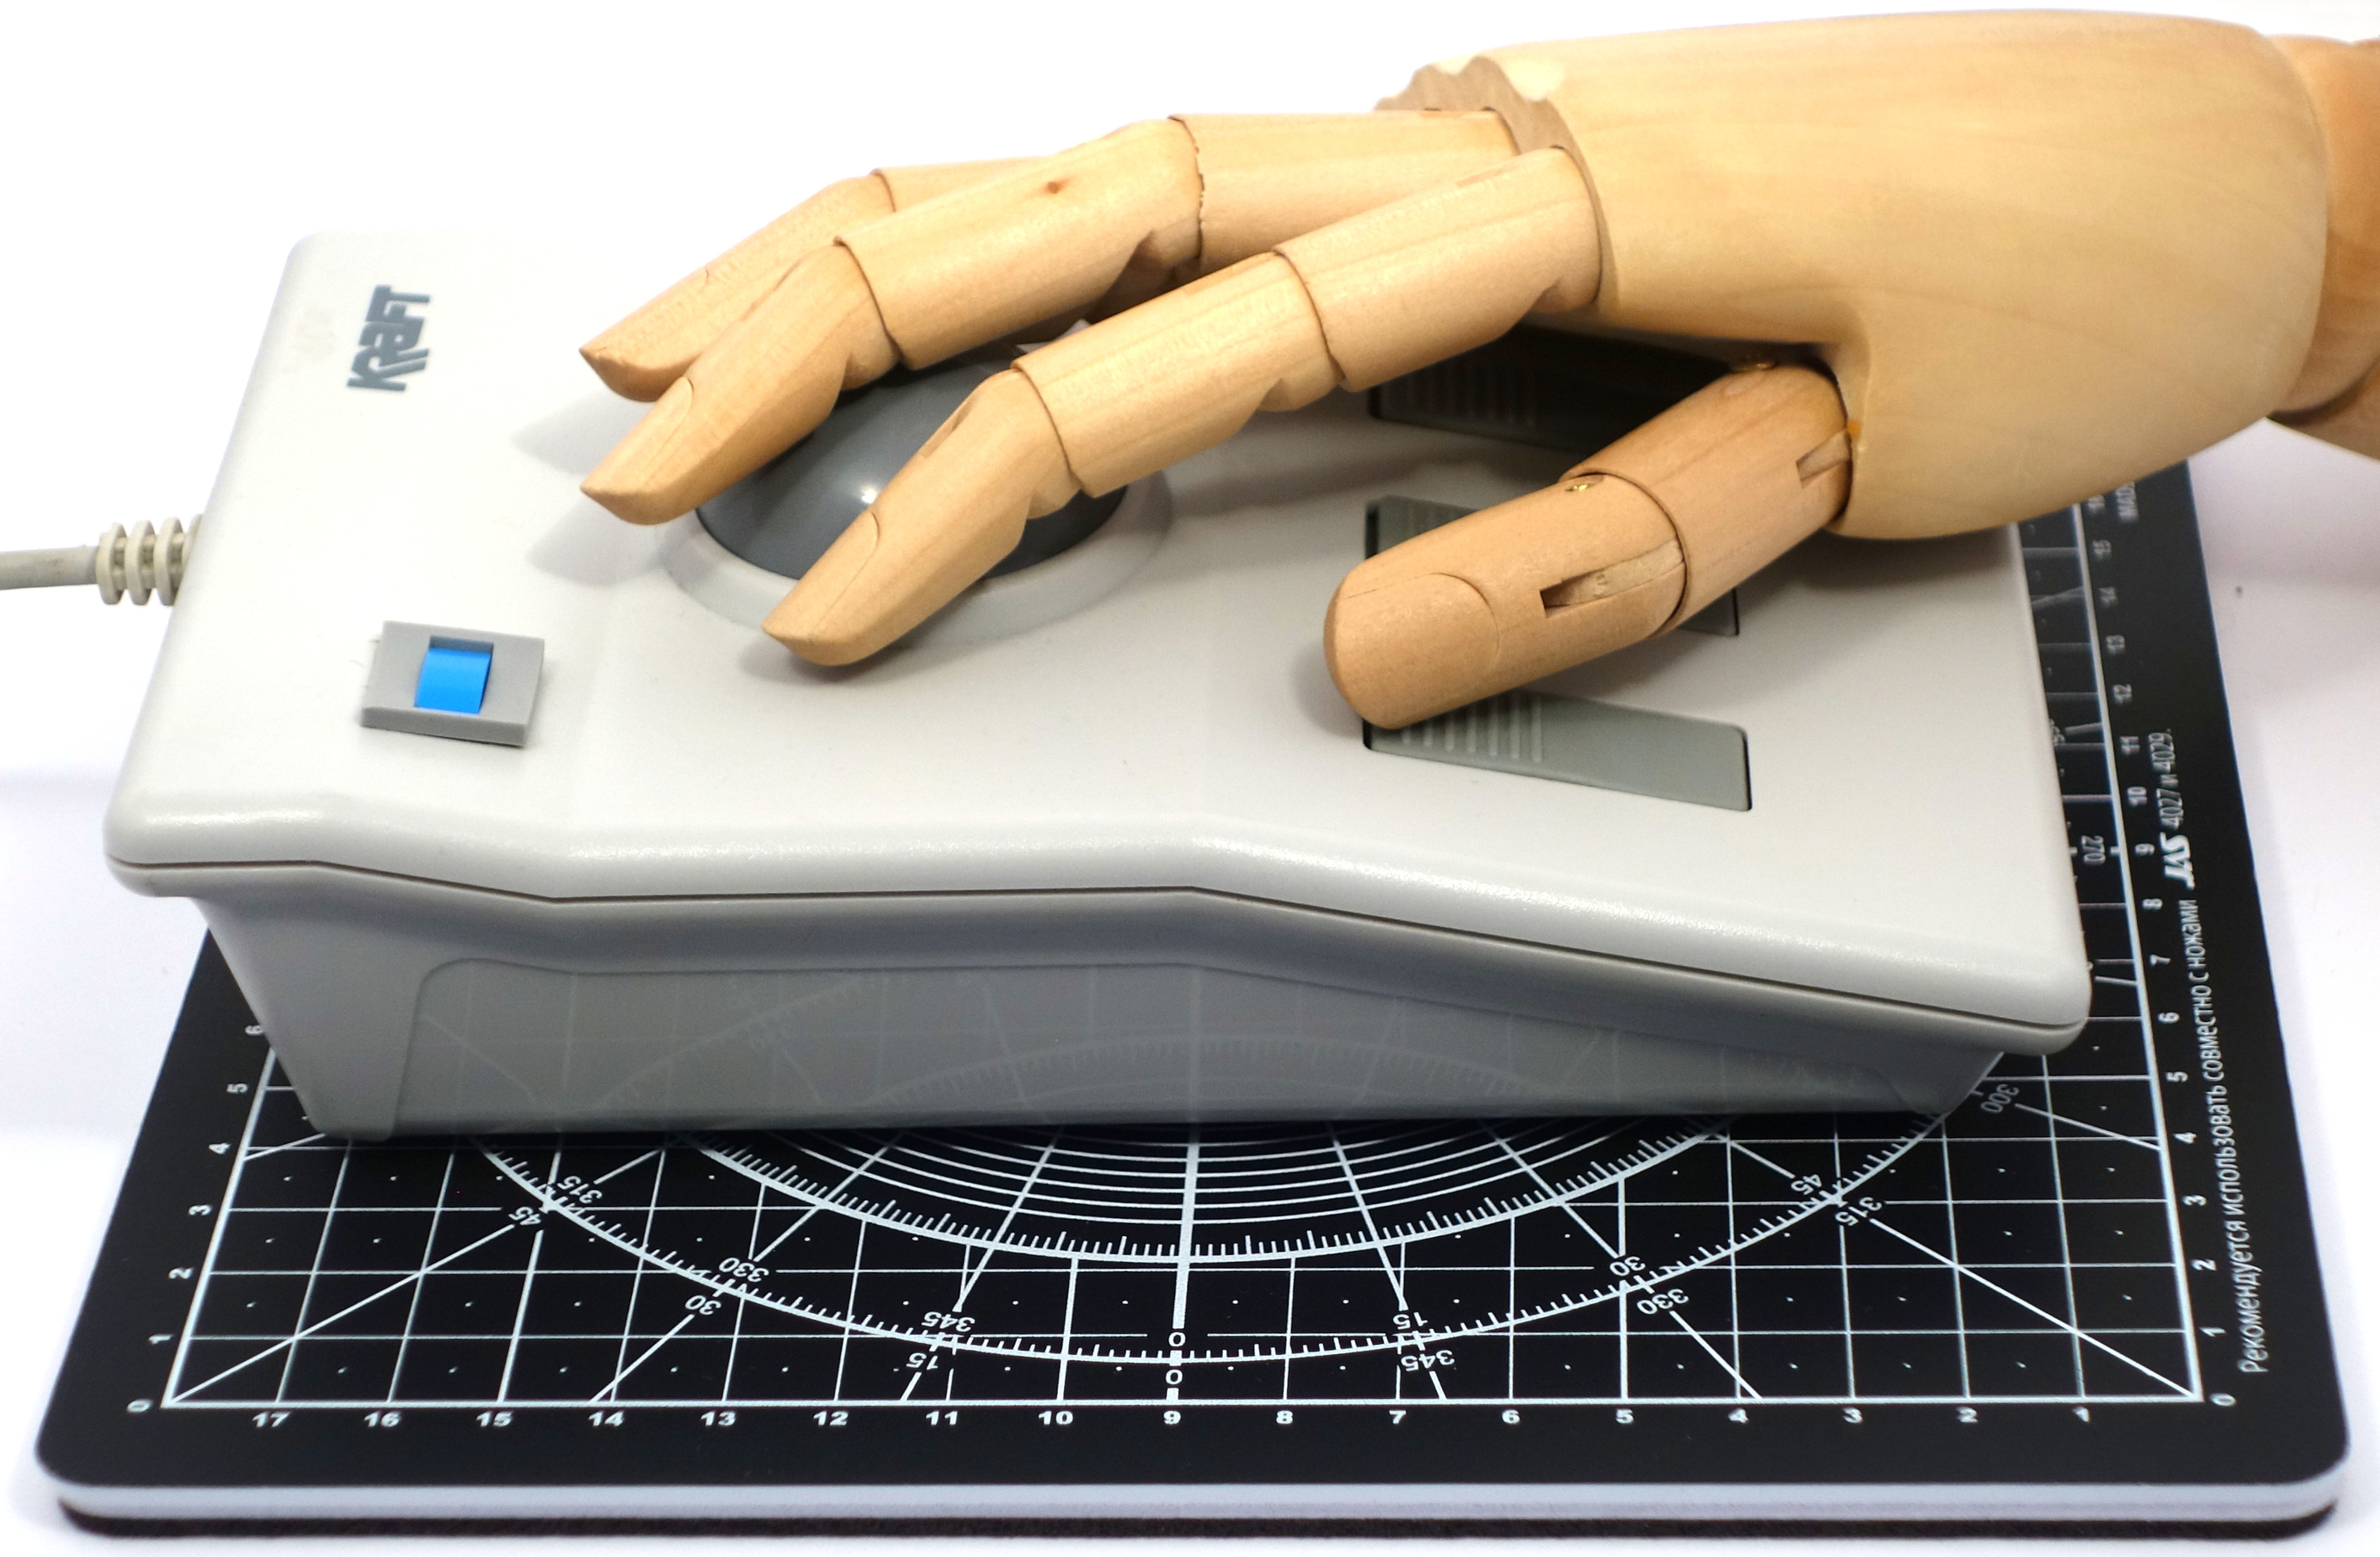
\includegraphics[scale=0.25]{1989_kraft_trackball/hand_30.jpg}
    \caption{Изображение Kraft trackball с моделью руки человека}
    \label{fig:KraftHand}
\end{figure}

Для облегчения операций перетаскивания объектов, а также выделения текста кликом и перетаскиванием, на устройстве предусмотрена четвертая кнопка, расположенная позади шара слева. Она срабатывает как левая кнопка, но реализована на базе переключателя с фиксацией, поэтому блокируется в нажатом состоянии до следующего нажатия. Расположение этой кнопки позволяет предположить что она рассчитана на нажатие указательным пальцем. Учитывая расположение, маленький размер и форму, нажимали ее не так часто.

Наиболее уникальным дополнительным аксессуаром трекбола Kraft является педаль (рис. \ref{fig:KraftPedal}). Она подключается к трекболу сзади с помощью стандартного телефонного кабеля с разъёмом RJ-11, и представляет собой металлическую прямоугольную коробку высотой в 1.5, шириной в 2 и длиной в 4 дюйма. Нажатие на педаль аналогично нажатию левой кнопки трекбола. Согласно обзору, представленному в \cite{kraftwithpedal}, в реальной эксплуатации педаль может практически полностью заменить левую кнопку.

\begin{figure}[h]
    \centering
    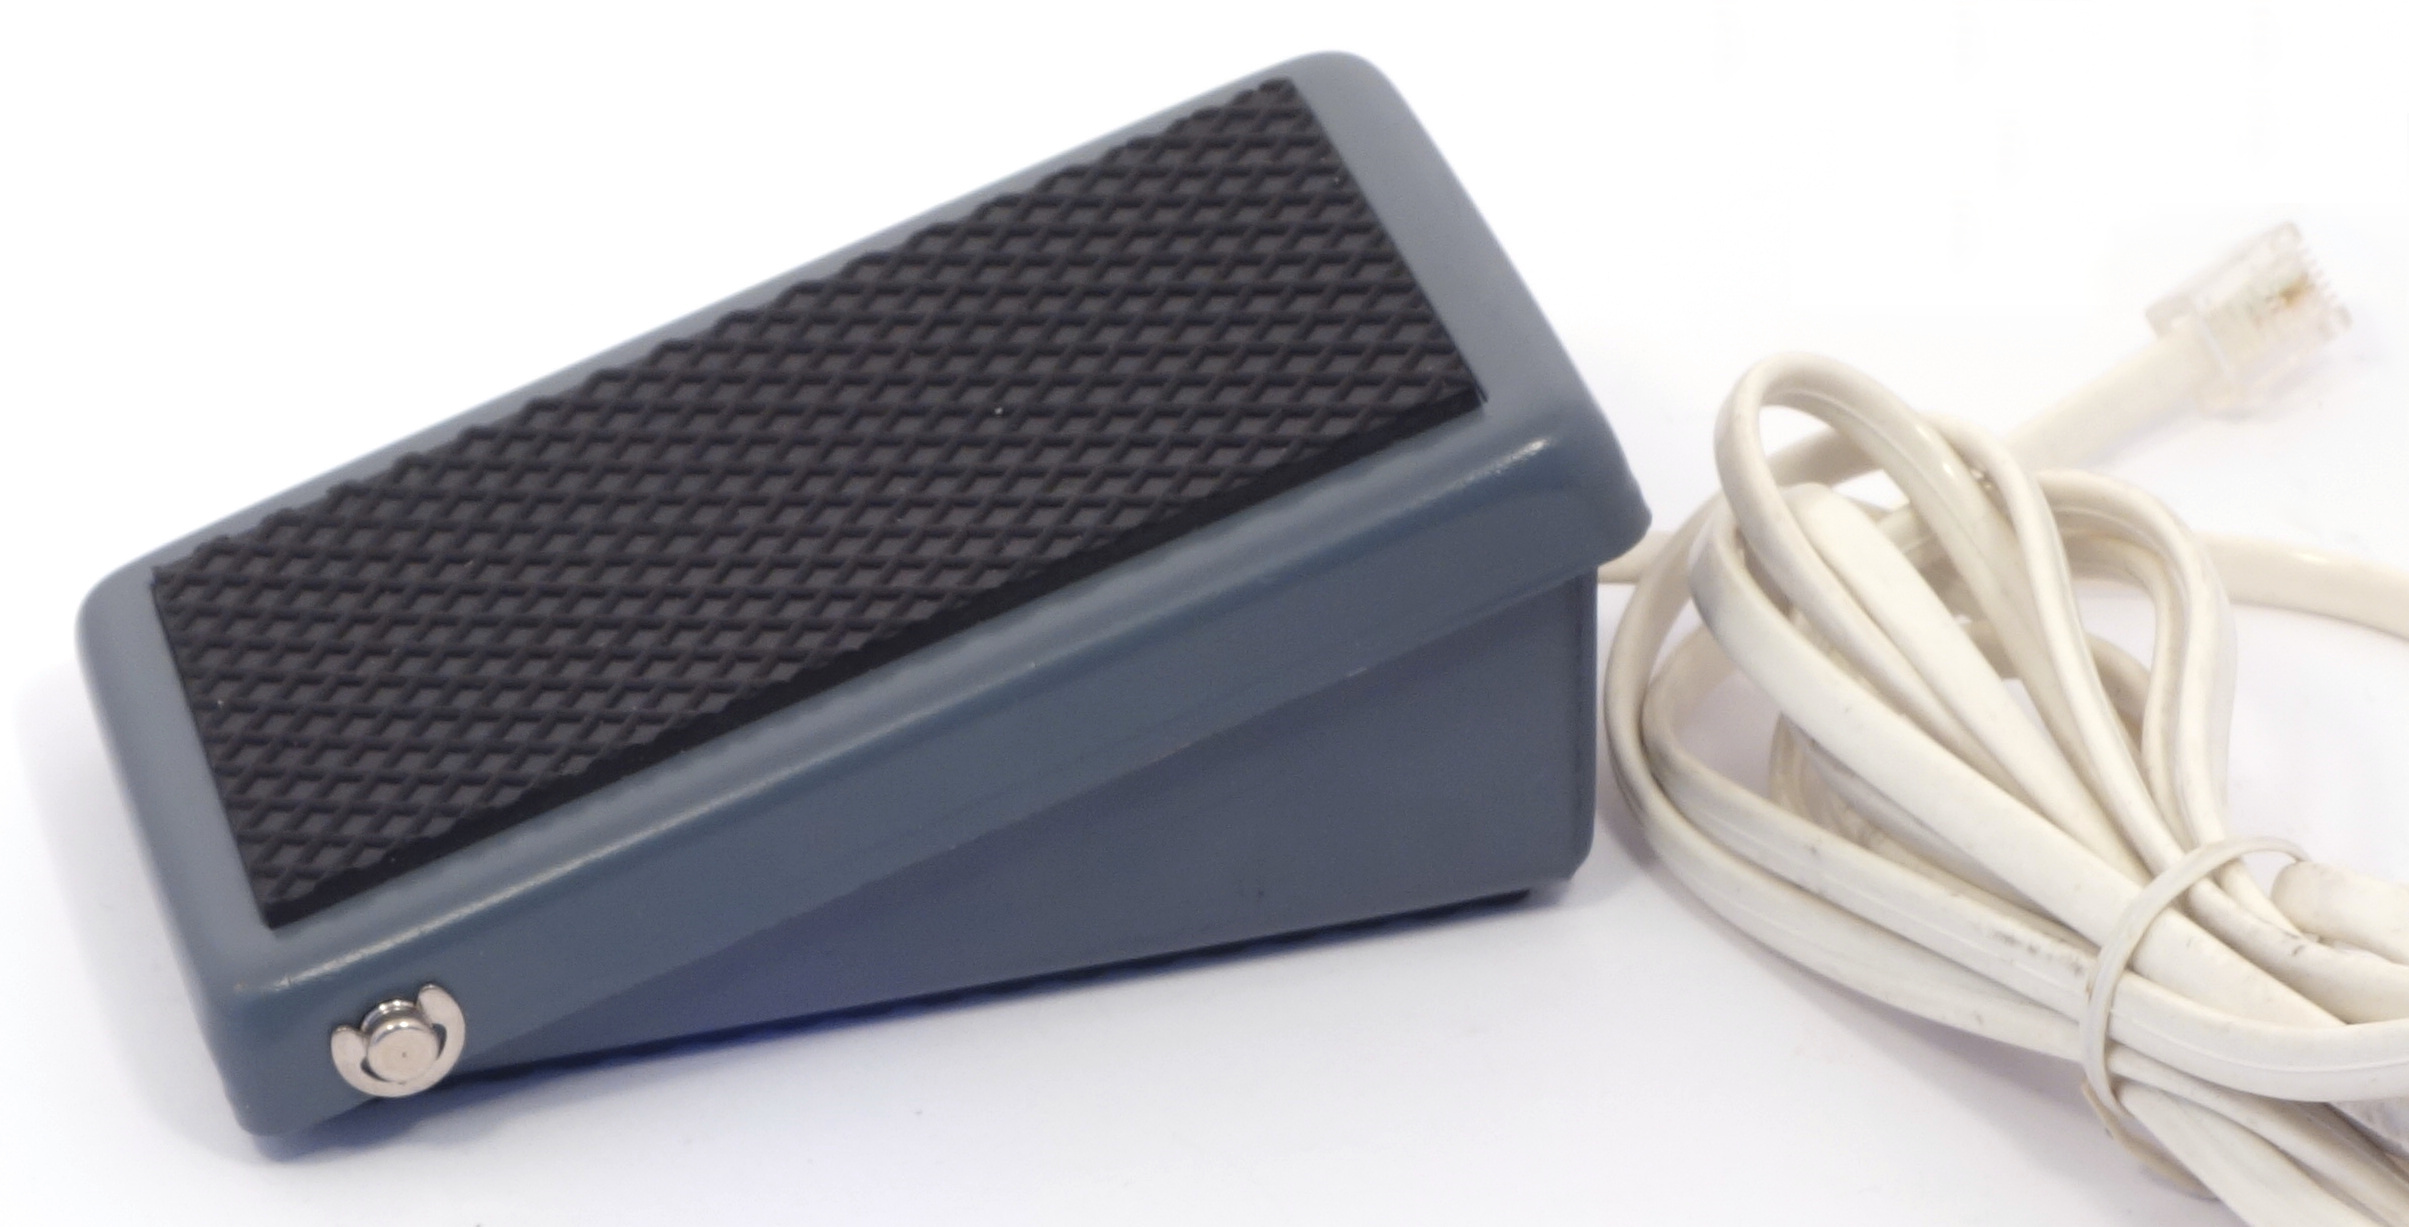
\includegraphics[scale=0.4]{1990_kraft_toptrack/pedal_30.jpg}
    \caption{Педаль Kraft trackball}
    \label{fig:KraftPedal}
\end{figure}

Вид трекбола в разобранном виде показан на рисунке \ref{fig:KraftInside}. Как можно видеть, технически это стандартное устройство позиционирования, выполненное по оптомеханической схеме. Проверка кода по базе данных Федеральной комиссии по коммуникациям США подтверждает, что трекбол был разработан американской компанией Kraft Systems в 1989 году.

\begin{figure}[h]
    \centering
    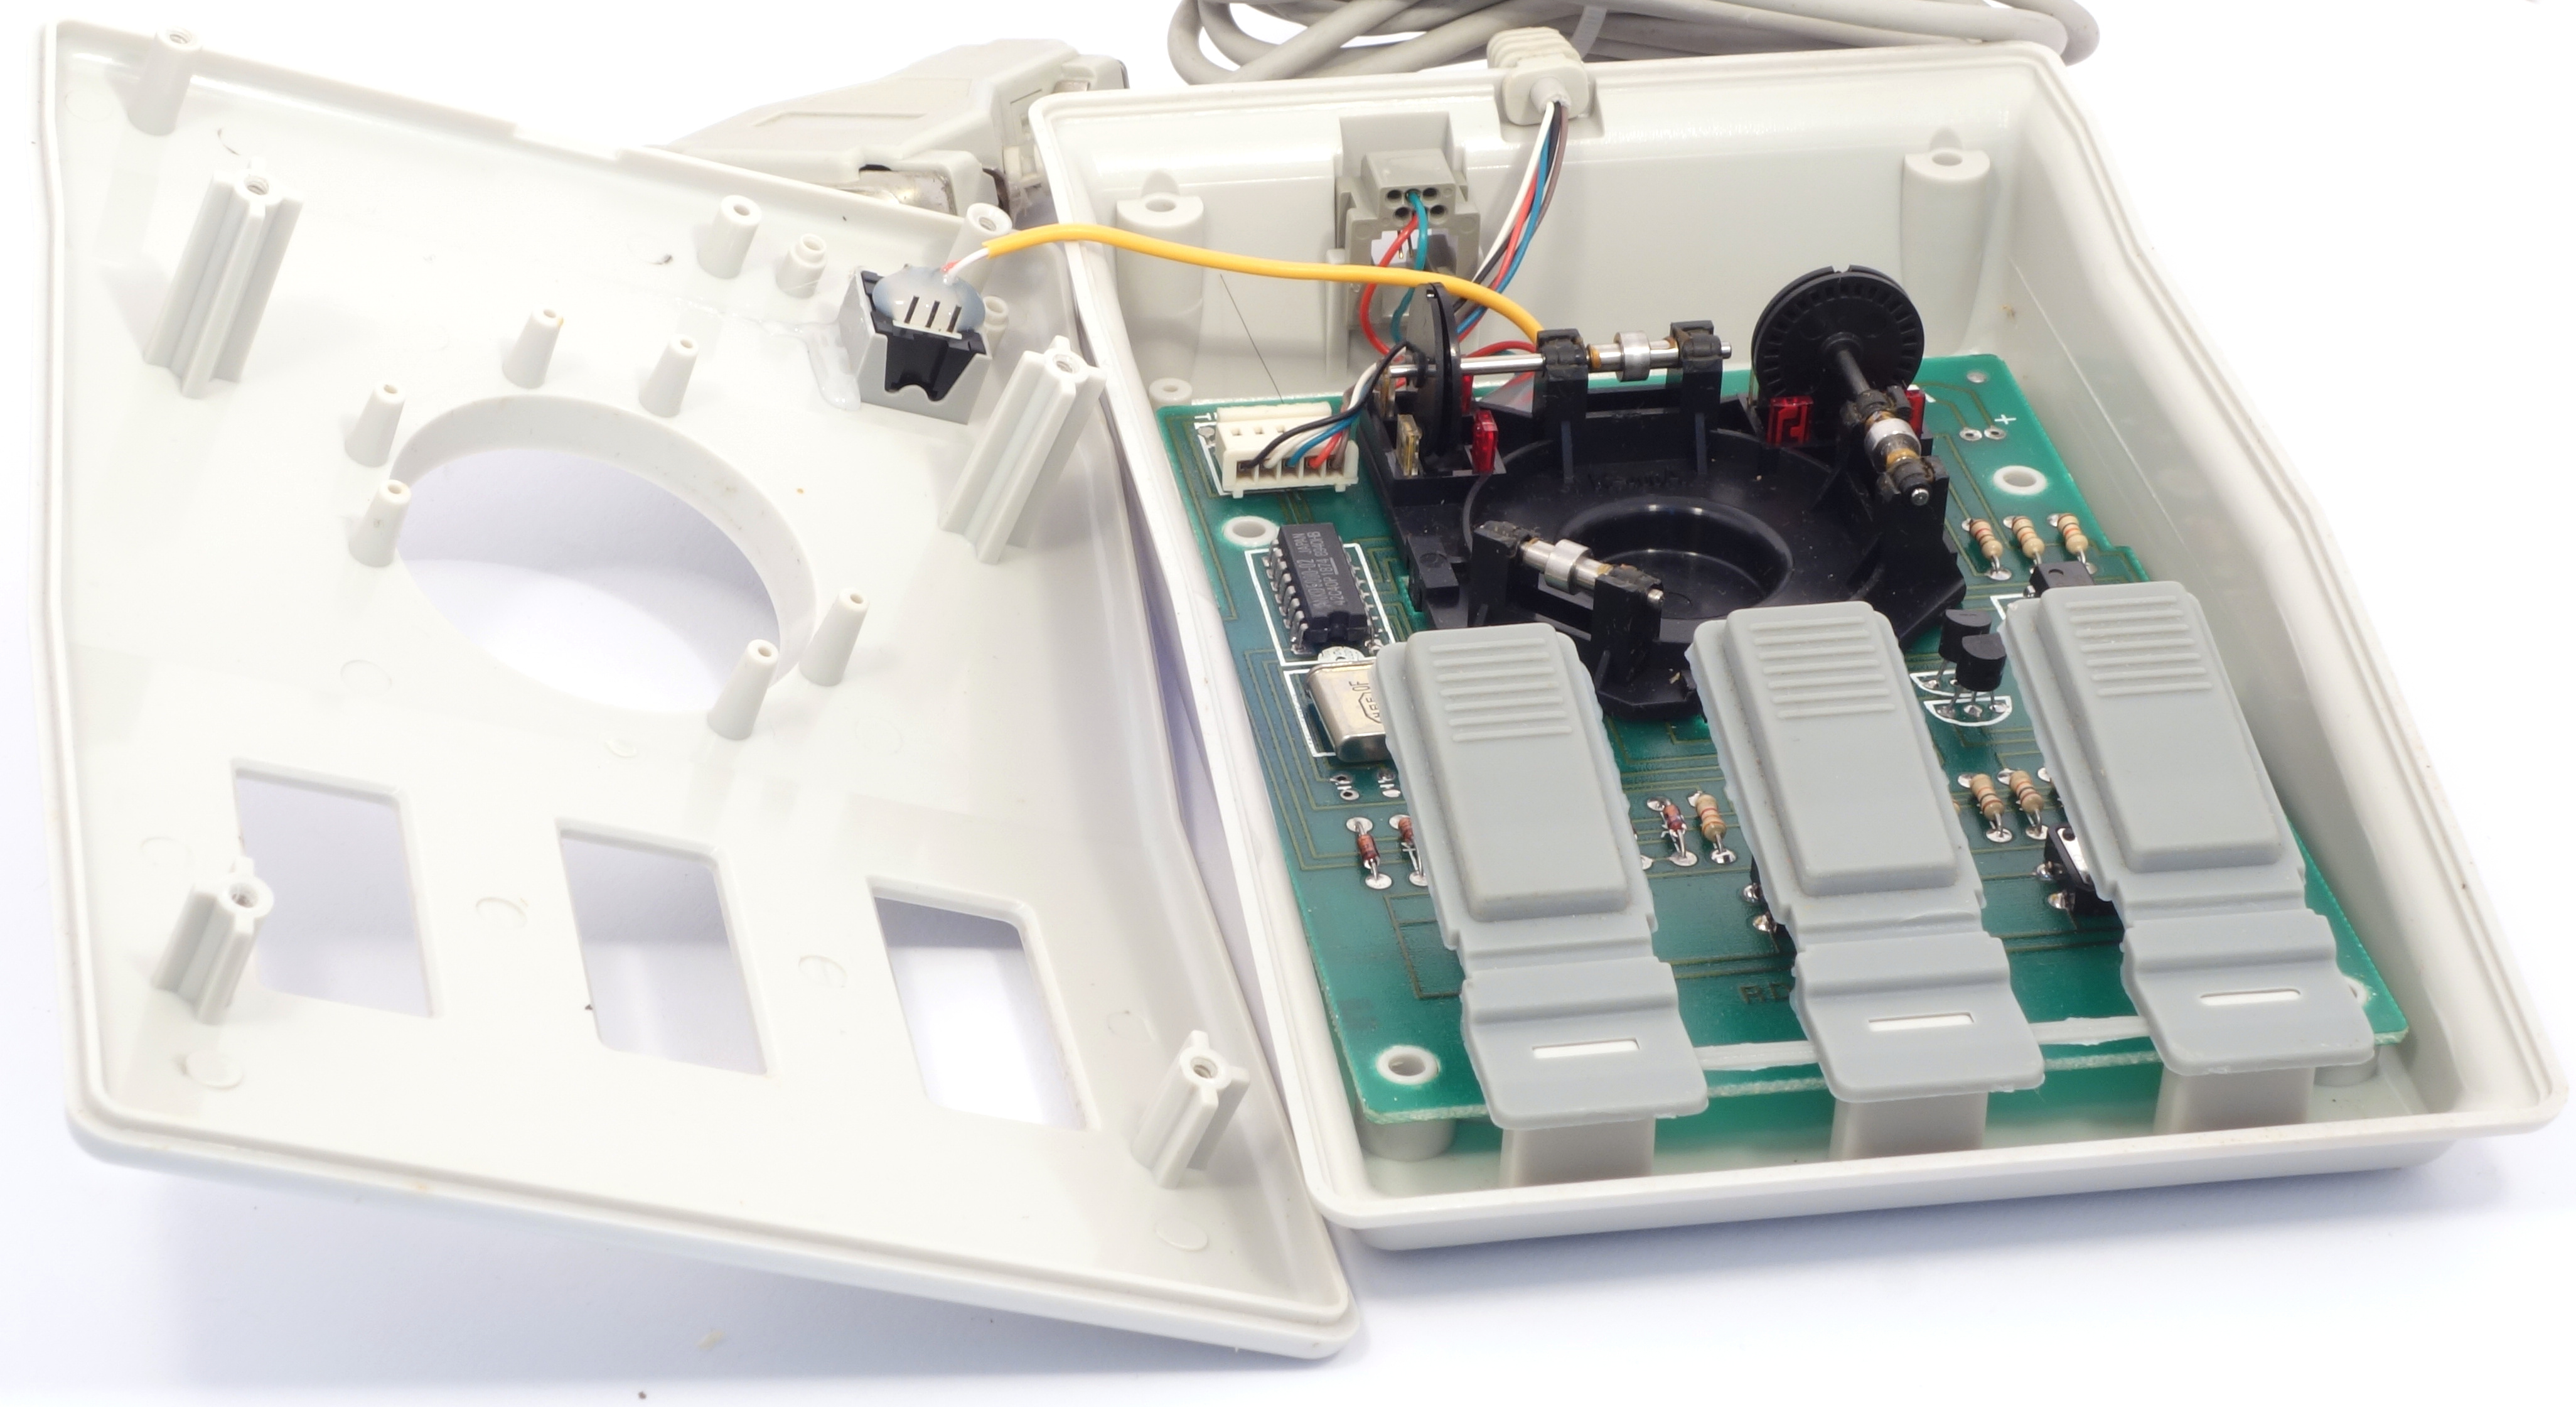
\includegraphics[scale=0.6]{1989_kraft_trackball/inside_30.jpg}
    \caption{Изображение Kraft trackball в разобранном виде}
    \label{fig:KraftInside}
\end{figure}

Программное обеспечение, поставляемое с трекболом, позволяет использовать его как с приложениями, управляемыми мышью, так и с приложениями, рассчитанными на управление с помощью клавиатуры. Драйвер позволяет настроить скорость, распознавание последовательных портов и некоторые другие элементы. Кроме того, трекбол Kraft можно использовать как с 9-контактным, так и с 25-контактным разъемом \cite{Hudnall}.

\begin{thebibliography}{9}
\bibitem{triple} Lennard V. Trackball Round-Up. ATARI/P\&G/CONTRIVER/MCS/MARCONI/KRAFT Trackballs // Music technology, December 1990. -- P. 42--47. \url{http://www.muzines.co.uk/articles/trackball-round-up/462}

\bibitem{Hudnall} Hudnall M. Kraft Trackball // Compute, August 1991. - P. 42. \url{https://www.atarimagazines.com/compute/issue132/42_Kraft_Trackball.php}

\bibitem{kraftwithpedal} Unger T. Kraft Trackball // PC Magazine, V. 9, No. 14, August 1990. - P. 249-251. \url{https://books.google.by/books?id=cSMUxSP5pKgC&lpg=PP1&pg=PT253#v=onepage&q&f=false}
\end{thebibliography}
\end{document} 
